\documentclass[UTF8]{ctexart}

\usepackage{subfiles}  

%下面的语句, 引入你的头部设置文件
\usepackage{C:/phpStorm_proj/02_myself_ID_EGO/+100_latex_all_math_sel/myPreamble} 
%必须是绝对路径,才能让各个tex在单独编译时使用到

\title{泰勒公式 Taylor Formula}


%---------------------------------



\begin{document}
\tableofcontents % 生成目录
\date{} % 若不写这句, 则默认也会渲染出日期, 所以我们要手动赋空值
\maketitle  %这行代码, 让你前面的 title, author, date生效



\part{泰勒公式  Taylor Formula}

泰勒函数的思想: 对于一个给定的光滑函数, 我们能否使用``任意次的多项式函数", 来逼近它?

事实上可以. 项数越多, 每项的系数不同, 多项式就能拟合不同的曲线.

$f\left( x \right) =a_0+a_1x+a_2x^2+a_3x^3+...$ \\

忽略系数后, 可以看到, 多项式最基础的部分, 就是幂函数 $x^1, x^2, ...$. \\

幂函数分为两种, 一种是"偶函数", 图像的开口方向同向: \\

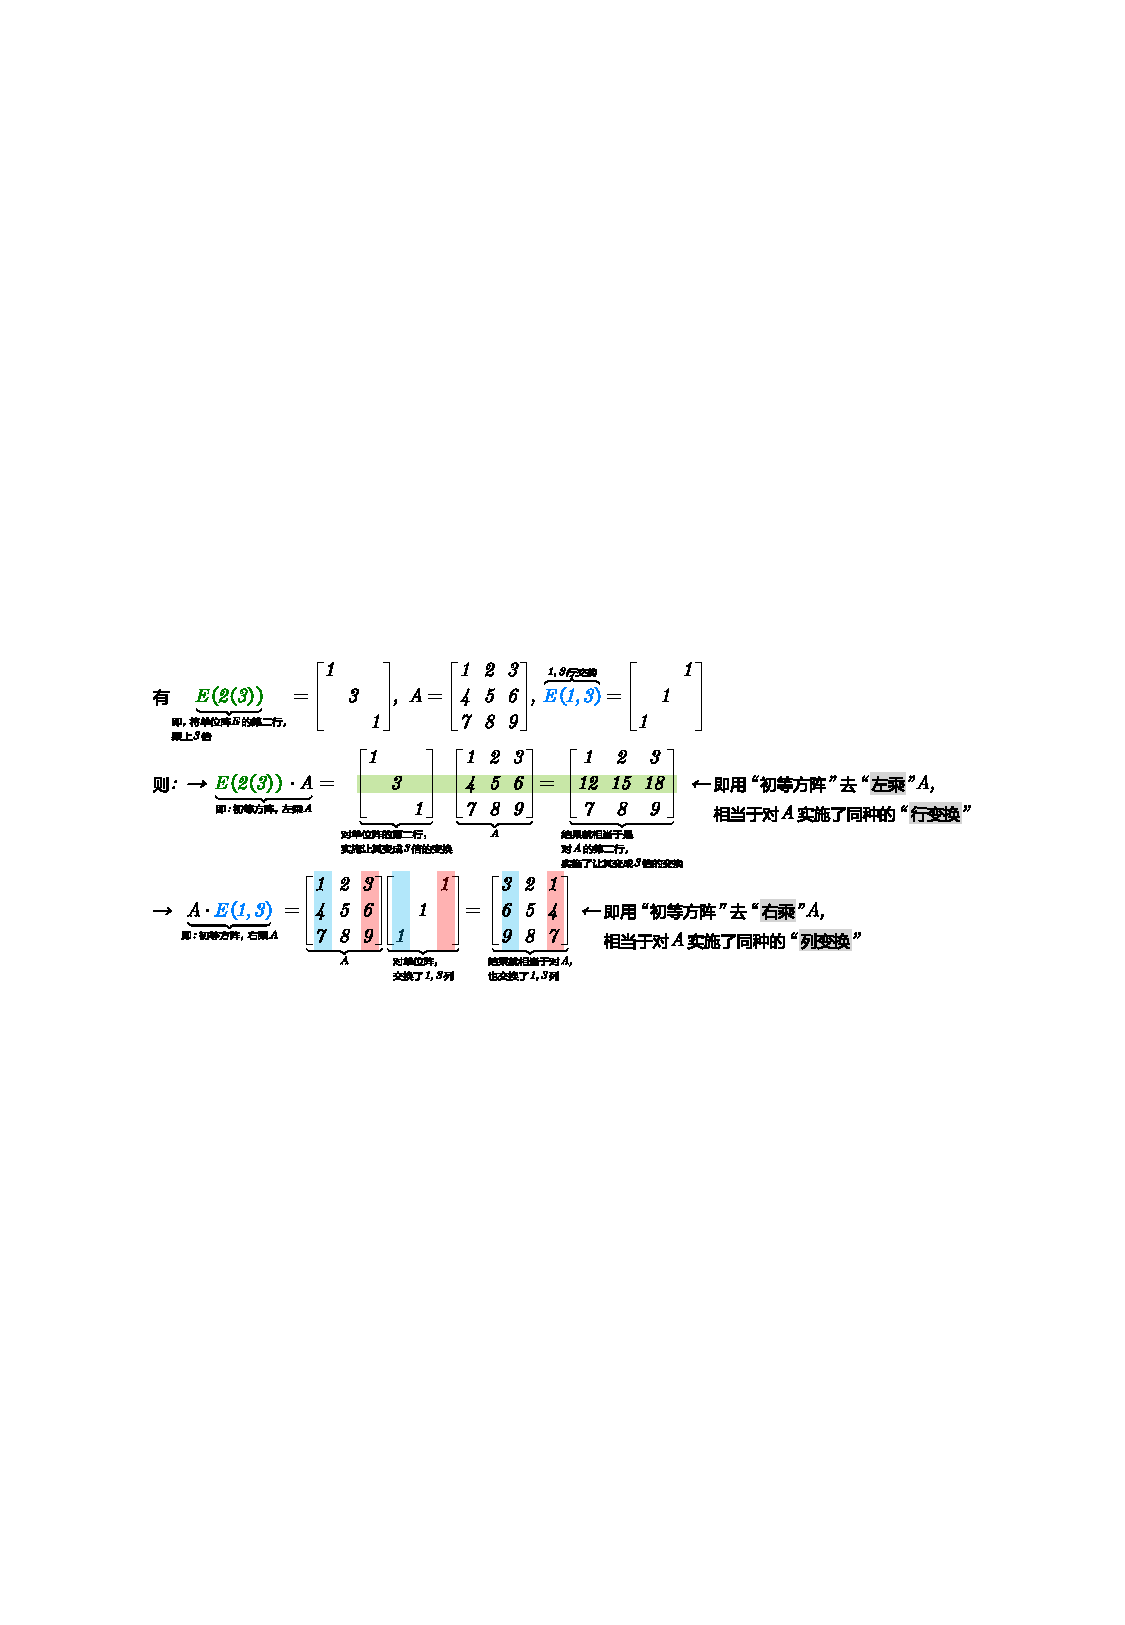
\includegraphics[width=0.5\textwidth]{/0036.pdf}

另一种, 为"奇函数", 图像的开口方向相反: \\

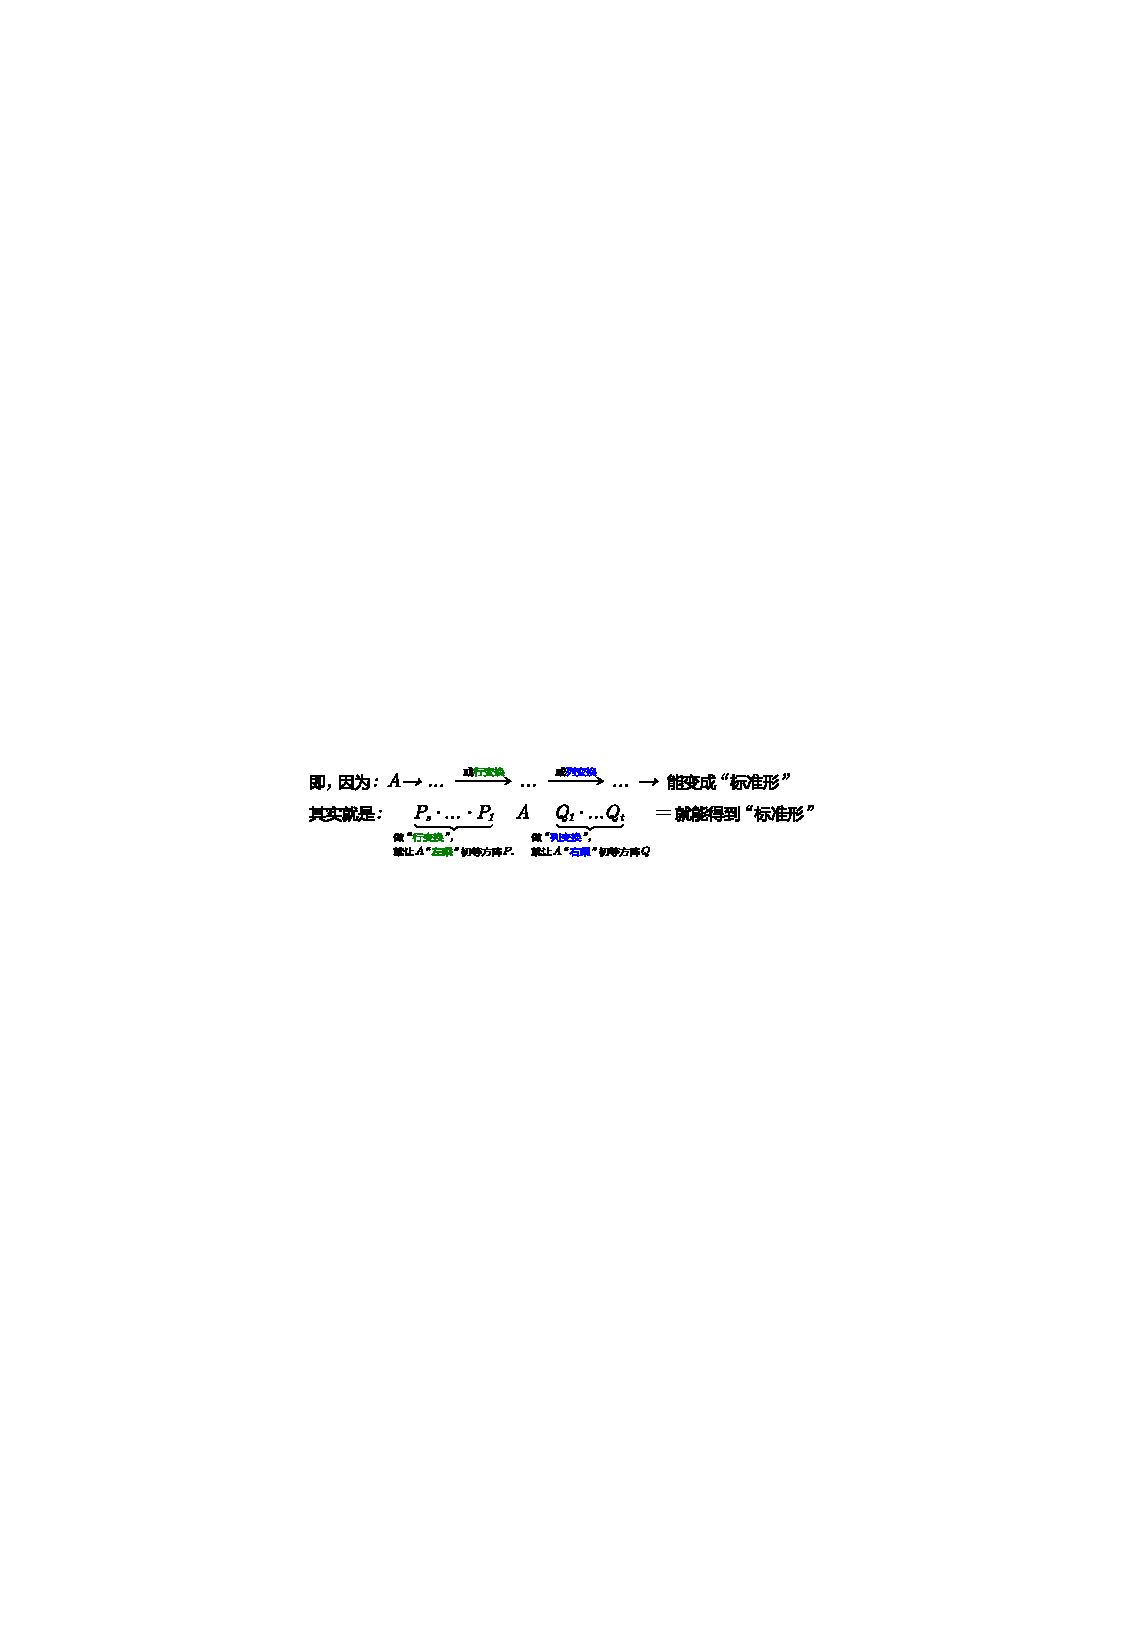
\includegraphics[width=0.5\textwidth]{/0037.pdf}

偶函数和奇函数组合在一起, 就能产生让曲线拉伸的效果.

泰勒公式的本质, 就是用``幂函数", 去``近似"任何一个函数. 反过来, 我们就可以把任何一个函数, 展开成``幂函数的和". \\

每个函数fn, 用泰勒展开后的前几项, 就是该函数fn的``等价无穷小"公式.

所谓``等价无穷小", 是指:  若 $\lim_{x \to x_0} \dfrac{f(x)} {g(x)} = 1$, 则称 f 和 g 是``等价无穷小量",记作 $f(x) \sim g(x) \quad (x \to x_0)$.


~\\
\hrule
~\\



\part{麦克劳林公式 Maclaurin's series}

泰勒公式, 我们一般在 $x_0 =0$ 处展开, 就变成麦克劳林公式(Maclaurin's series), 它是泰勒公式的一种特殊形式. \\

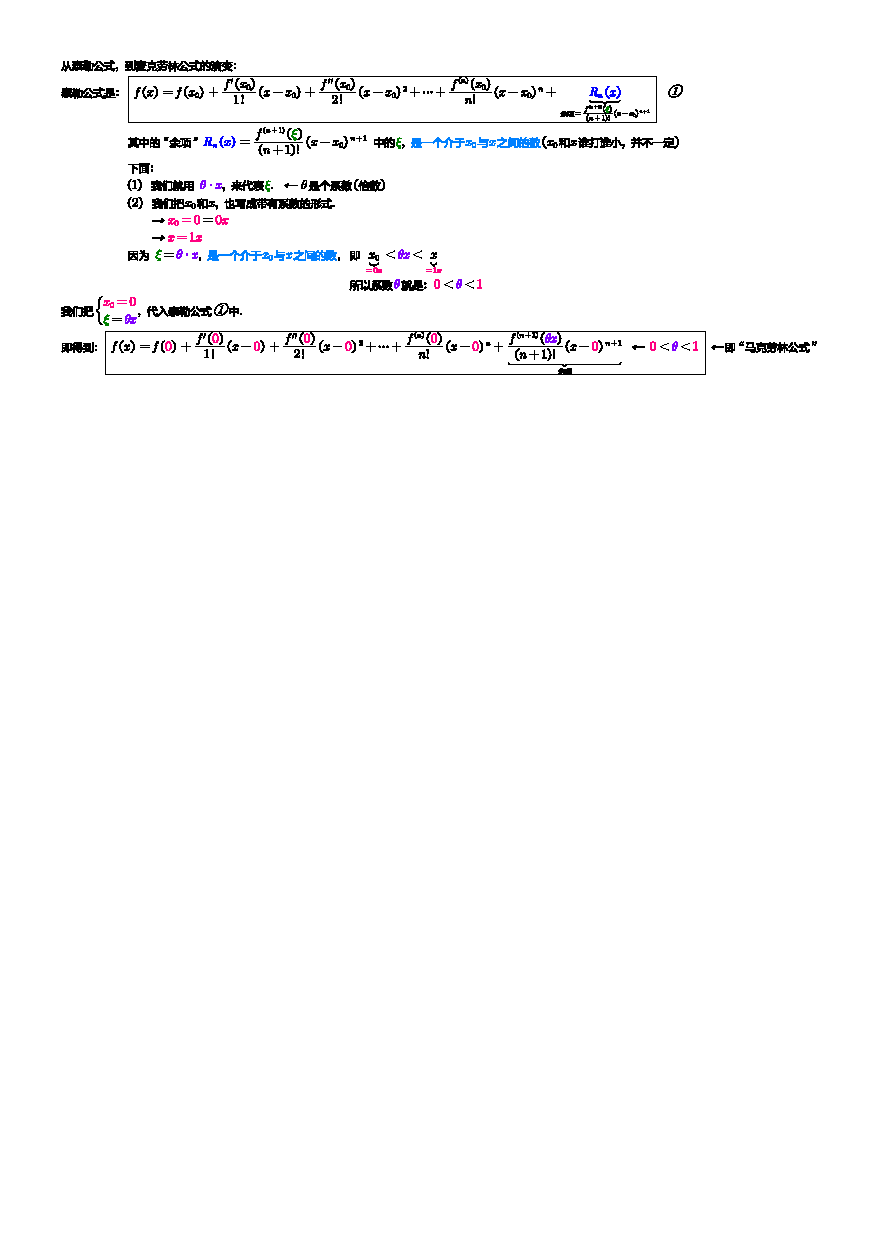
\includegraphics[width=1\textwidth]{/0038.pdf}

\textbf{注意: 余项的分子上的 $f^{\left( n+1 \right)}\left( \theta x \right) $, 意思是 对 $f(\theta x)$ 函数 求 n+1 次导数 (而不是次方的意思, 别搞错了).}


麦克劳林公式, 比泰勒公式更常用. 即, 我们一般只在 $x_0=0$ 处展开泰勒公式. \\


\begin{myEnvSample}
	对 $f(x)=e^x$ 用马克劳林公式来拟合它 (在 $x_0 = 0$点处展开)
	
	\textbf{那我们就把 $e^x$ 代入``马克劳林公式"中的分子上的每个f 中了.} \\
	
	\boxed{
		\text{麦克劳林公式: } f\left( x \right) =f\left( 0 \right) +\frac{f'\left( 0 \right)}{1!}x + \frac{f''\left( 0 \right)}{2!}x^2 + \cdots +\frac{f^{\left( n \right)}\left( 0 \right)}{n!}x^n + \text{余项} \frac{f^{\left( n+1 \right)}\left( \theta x \right)}{\text{(}n+1\text{)!}}x^{n+1}
	} \\

	本例的f 代入后, 就是: 	
	\begin{align*}  % 支持每行编号. 若不需要编号, 就用 align*环境
			 e^x &= e^0+\frac{\left( e^0 \right) '}{1!}x+\frac{\left( e^0 \right) ''}{2!}x^2+...+\frac{\left( e^0 \right) ^{\left( n \right) \text{次导数}}}{n!}x^n+\text{余项}\frac{\left( e^{\theta x} \right) ^{\left( n+1 \right) \text{次导数}}}{\left( n+1 \right) !}\left( x \right) ^{n+1}\\
			& =1+x+\frac{1}{2!}x^2+...+\frac{1}{n!}x^n+\frac{e^{\theta x}}{\left( n+1 \right) !},\ \ \ 0<\theta <1		
	\end{align*}
	
上面, 因为 $e^x$ 的任何次导数, 都等于 $e^x$ 自己. 所以在$x_0 = 0$处展开后, 上面的每一个分子上, 就有: $\left( e^0 \right) '=\left( e^0 \right) ''=...=\left( e^0 \right) ^{\left( n \right) \text{次导数}} =1$ \\

\end{myEnvSample}



注意: 只要用``麦克劳林公式"来拟合, 就一定能得到严格的``等于号(=)", 而不是约等于号($\approx$). \textbf{因为余项中的$\theta$ 所取的区间 0-1 之中, 一定能取到一个数, 能令``麦克劳林公式"能精确的拟合原函数. 但至于$\theta$ 到底是哪个数? 我们是不知道的.} \\

反过来说, 如果你把余项部分去掉了, $\theta$ 就不存在了. 则就只能使用约等于号($\approx$)了. \\


即, 去掉余项后, 上例就是: 
\begin{align*}  % 支持每行编号. 若不需要编号, 就用 align*环境
	e^x & \approx e^0+\frac{\left( e^0 \right) '}{1!}x+\frac{\left( e^0 \right) ''}{2!}x^2+...+\frac{\left( e^0 \right) ^{\left( n \right) \text{次导数}}}{n!}x^n\\
	& \approx 1+x+\frac{1}{2!}x^2+...+\frac{1}{n!}x^n  
\end{align*}



\begin{myEnvSample}
	又例如, 我们用 马克劳林公式, 来拟合 $ f(x) = \sin x$.
	
	即, 把 sin x 的各次导数, 代入马克劳林公式的每个分子上. \\ 
	
	$\left( \sin x \right) '=\cos x$ ← 因为公式是在 x=0 处展开, 即把 x=0 代进去, 即 $\left( \sin 0 \right) '=\cos 0=1$
	
	$\left( \sin x \right) ''=-\sin x\ \ \ \gets \left( \sin 0 \right) ''=-\sin 0=0$
	
	$\left( \sin x \right) ^{\left( 3 \right)}=-\cos x\ \ \ \gets \left( \sin 0 \right) ^{\left( 3 \right)}=-\cos 0=-1$
	
	$\left( \sin x \right) ^{\left( 4 \right)}=\sin x\ \ \ \gets \left( \sin 0 \right) ^{\left( 4 \right)}=\sin 0=0$ \\
	
	我们可以发现 sin x 的高阶导数的规律:  
	
	→ 其偶数阶导数 = 0
	
	→ 当 x=0 时, 其高阶导数的导数值, 以 1, 0, -1, 0 循环 \\
	
	下面, 就把 sin 这些各次的导数值, 代入马克劳林公式中.
	
	马克劳林公式是: 
	
	$ f\left( x \right) =f\left( 0 \right) +\frac{f'\left( 0 \right)}{1!}\left( x-0 \right) +\frac{f''\left( 0 \right)}{2!}\left( x-0 \right) ^2+\cdots +\frac{f^{\left( n \right)}\left( 0 \right)}{n!}\left( x-0 \right) ^n+\underset{\text{余项}}{\underbrace{\frac{f^{\left( n+1 \right)}\left( \theta x \right)}{\left( n+1 \right) !}\left( x-0 \right) ^{n+1}}}	$
	
	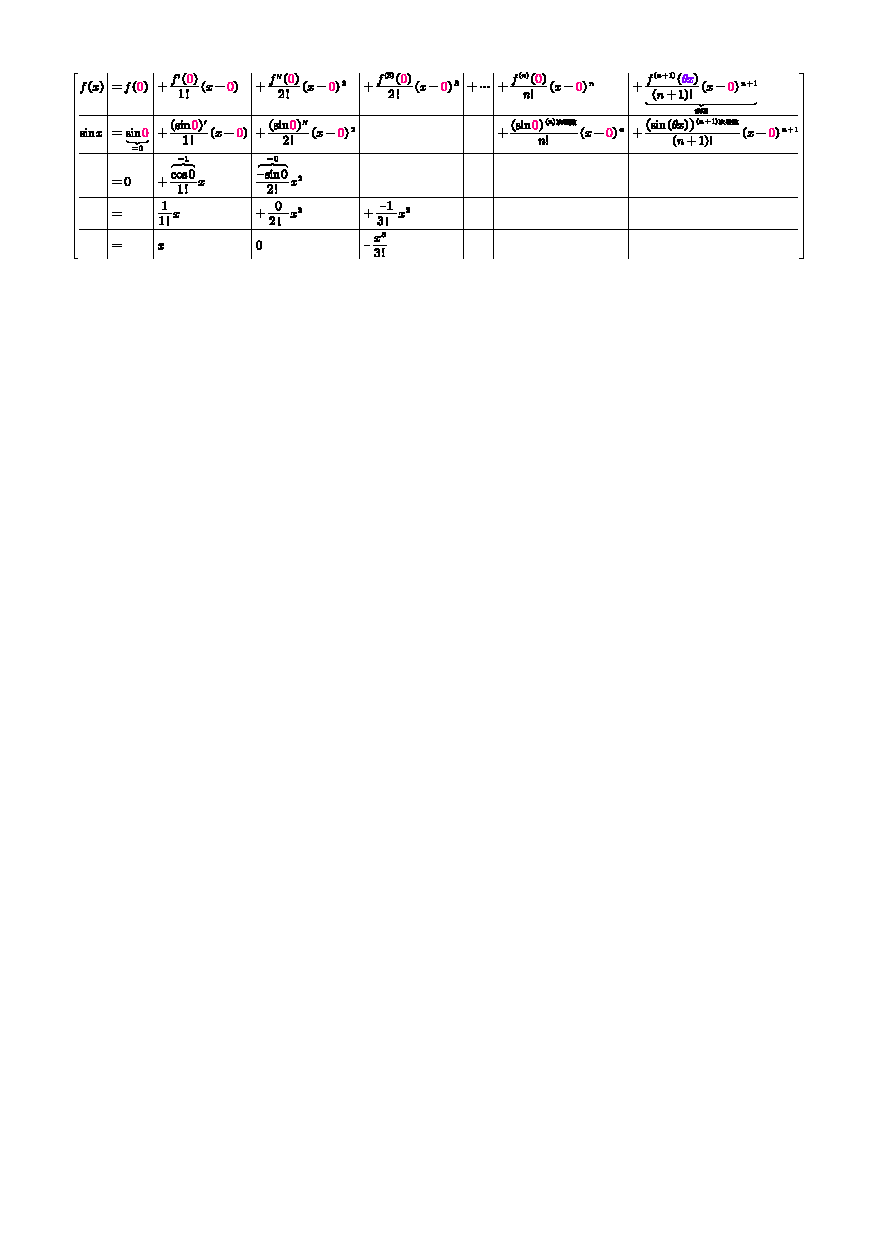
\includegraphics[width=1\textwidth]{/0039.pdf}
	
	所以 sin x 展开后, 就是: \\
	
	$\sin x=x-\frac{x^3}{3!}+\frac{x^5}{5!}-\frac{x^7}{7!}+...+\left( -1 \right) ^n\frac{x^{2n+1}}{\left( 2n+1 \right) !}+o\left( x^{2n+2} \right) =\sum_{k=0}^{\infty}{\frac{\left( -1 \right) ^k}{\left( 2k+1 \right) !}x^{2k+1}}
	 $ \\
	
	所以, 如果只取第一项, 就有 $ \sin x \sim x$ \\
	
	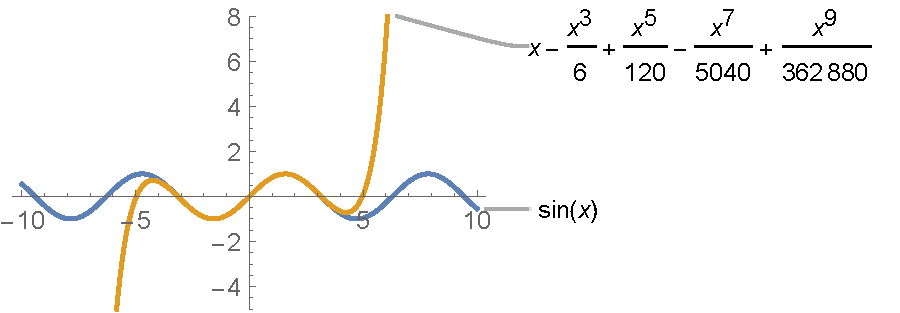
\includegraphics[width=0.6\textwidth]{/0040.pdf}
	
\end{myEnvSample}





\end{document}